\section{Brugergrænseflade}
\label{sec:webapplikationen}

Som resultat af prototypeafprøvningerne med informanter, som er beskrevet i afsnittene \ref{subsec:prototype1} og \ref{subsec:prototype2}, følger her en præsentation og beskrivelse af den endelige brugergrænseflade. Vi har udviklet en webapplikation, som vi har valgt at kalde \Foodl{}.

\subsection{Forside}
\label{subsec:brug-forside}

Når man taster sig ind på hjemmesiden \url{http://www.foodl.dk}, bliver man mødt af en velkomsthilsen, der meget kort beskriver hjemmesidens formål og brug, som kan ses på \figref{fig:overblik-forside}. Denne hilsen kan brugeren vælge at lukke ned. En cookie bliver gemt i browseren, så velkomsthilsnen ikke bliver vist igen, medmindre browserhistorikken bliver ryddet.

\begin{figure}[H]
	\centering
	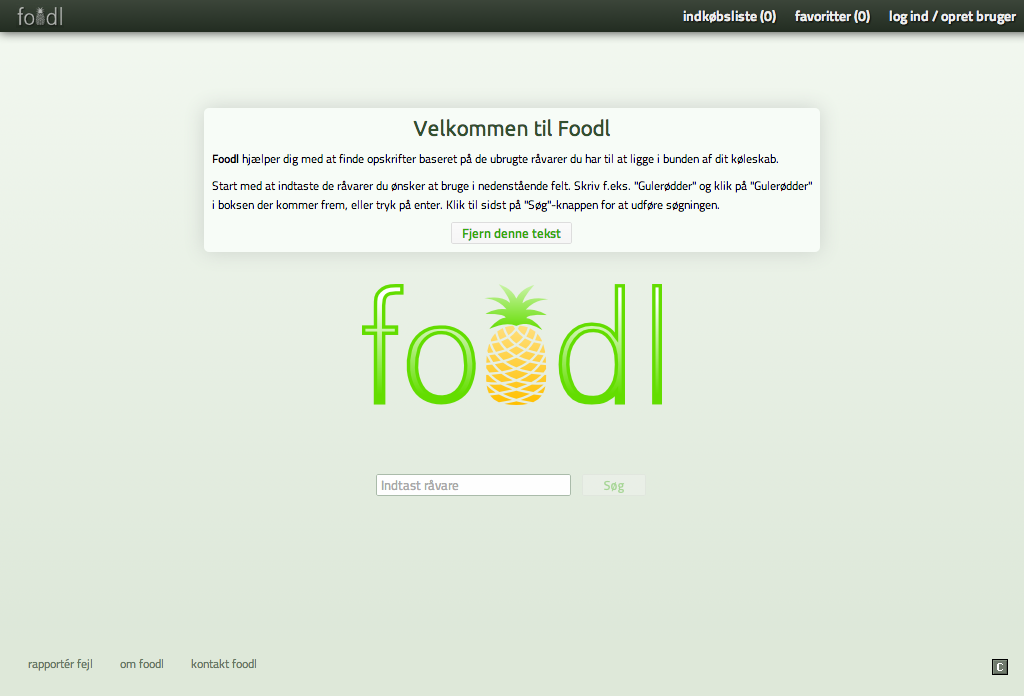
\includegraphics[scale=1]{billeder/foodl/thumbnails/forside.png}
	\capt{Denne figur har til formål at give et overblik over systemets forside.}
	\label{fig:overblik-forside}
\end{figure}

Navnet \Foodl{} er også en del af webapplikationens logo. For at gøre det klarere for en ny bruger, hvad siden handler om, erstattede vi et O i navnet med en stor ananas, fordi det er noget, der kan spises, og sidens formål er at give folk mulighed for at genbruge deres madrester. 

På toppen af alle undersider af \Foodl{} er det muligt at tilgå sidehovedet. Her er der mulighed for at navigere tilbage til forsiden ved at klikke på den mindre version af det store logo. Derudover kan man tilgå både en indkøbsliste, der er nærmere beskrevet i \secref{subsec:brug-indkoebsliste}, og en liste af favorit-opskrifter, som brugeren selv vælger fra hjemmesiden. Favoritlisten bliver beskrevet nærmere i \secref{subsec:brug-favoritliste}. Både indkøbslisten og favoritter har et tal i parentes, der fortæller brugeren, hvor mange varer, der er i den nuværende indkøbsliste, eller hvor mange opskrifter, der er gemt under favoritter. Dette kan ses påtoppen af \figref{fig:overblik-forside}. På sidehovedet kan man også logge ind i systemet eller oprette en bruger, hvilket er forklaret nærmere i \secref{subsec:brug-brugeroprettelse}.

Efter brugeren føler sig tryg ved hjemmesiden og evt. har lukket velkomsthilsnen ned, så er det tid til at indtaste alle de råvarer, der ønskes brugt til madlavningen. Figur \ref{fig:foodl-soegefelt} viser, hvordan en sådan søgning foregår. Der bliver løbende indtastet bogstaver, og systemet undersøger for dele af tekststrenge, der matcher det, som bliver indtastet. Ud fra disse match gives der forslag til hvilke råvarer, man kan vælge. Man kan ikke indtaste, hvad som helst som et søgekriterie i systemet. Der er en lang række råvarer at vælge imellem. Hvis der \fx bliver indtastet kød i søgefeltet, så kommer der en liste af matchende råvarer som forslag, som man kan se på \figref{fig:foodl-soegefelt}. Der er ingen begræsning for, hvor mange råvarer, der kan indtastes som søgekriterier.

\begin{figure}[H]
	\centering
	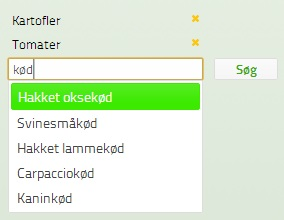
\includegraphics[scale=0.7]{billeder/foodl/soegefelt.jpg}
	\capt{Denne figur viser systemets søgefelt.}
	\label{fig:foodl-soegefelt}
\end{figure}


For at fuldføre en søgning skal man blot trykke på ``Søg'', der er til højre for søgefeltet. Når brugeren trykker ``Søg'', så arbejder systemet på at finde alle de opskrifter, der minimum har én ingrediens, der matcher en af de indtastede råvarer. Det er efter sådan en søgning, at brugeren finder ud af, hvad der er muligt at lave ud fra de råvarer, der er til rådighed (resultatet er afgrænset til den database, man har over opskrifter).
\subsection{Resultatside}
\label{subsec:brug-resultat}

Når en søgning bliver udført, så bliver brugeren navigeret videre til søgeresultatsiden, hvor man får præsenteret en liste af opskrifter, der matcher de søgekriterier, der er blevet skrevet ind i søgefeltet. Figur \ref{fig:overblik-resultat} giver et overblik over, hvordan sådan en liste kan se ud.

\begin{figure}[ht]
	\centering
	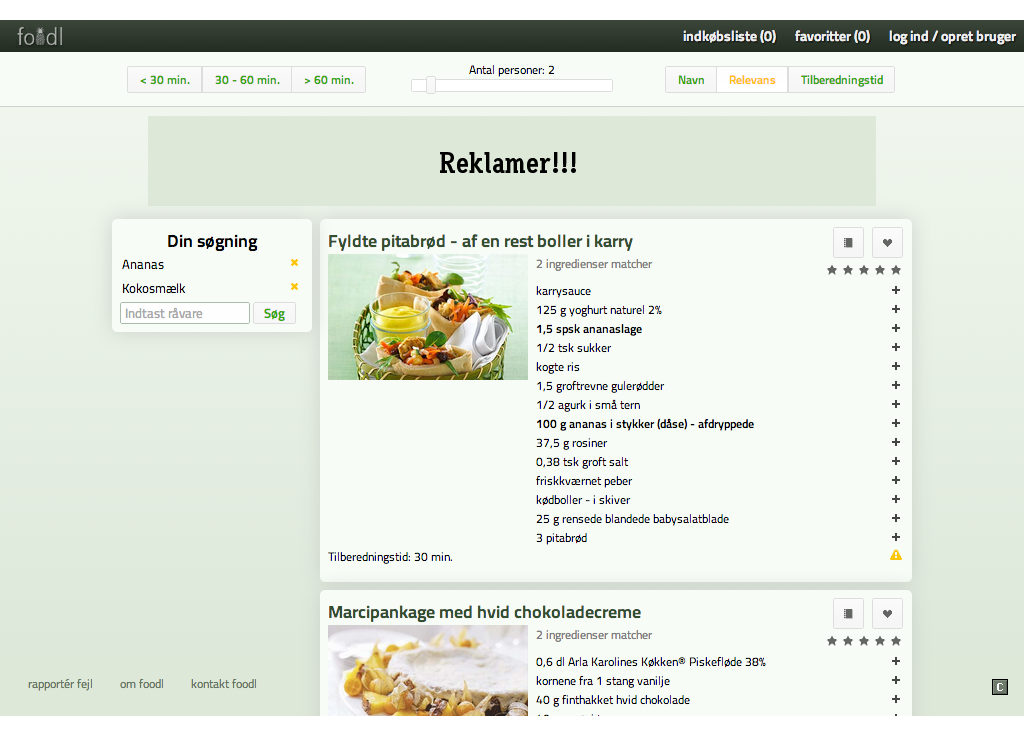
\includegraphics[scale=1]{billeder/foodl/thumbnails/soegeresultat.png}
	\capt{Denne figur har til formål at give et overblik over systemets resultatside.}
	\label{fig:overblik-resultat}
\end{figure}

I første omgang er opskrifterne sorteret efter relevans, dvs. hvor mange ingredienser, der matcher de forskellige indtastede råvaretyper. Figur \ref{fig:overblik-resultat} viser et eksempel af, hvordan sådan en liste ser ud. De ingredienser, der matcher søgekriterierne bliver markeret med fed skrift. 

På hjemmesiden vises der kun hvilke ingredienser, der skal til for at lave opskriften, men selve fremgangsmåden er ikke vist nogen steder. Man er nødt til at tilgå den oprindelige hjemmeside, hvorfra opskriften stammer fra. Dette gøres ved at trykke på enten opskriftens titel eller billedet. Begge elementer består af et link til opskriftens originale hjemmeside. 

Opskrifternes fremgangsmåde kan ikke ses på \Foodl{}, men alle andre vigtige elementer af opskriften er synlige. En opskrift består af følgende elementer:

\begin{itemize}[noitemsep]
\item Titel
\item Billede
\item Tilberedningstid
\item Relevans (antal matchende ingredienser)
\item Ingredienser
\item Knapper
\begin{itemize}[noitemsep]
\item Tilføj alle ingredienser til indkøbsliste
\item Tilføj / fjern fra favoritter
\item Tilføj enkelte ingredienser til indkøbsliste
\item Indmeld en fejl med opskriften
\end{itemize}
\end{itemize}

Alle opskrifter består af en beskrivende titel og et relevant billede, der skal vise brugeren, hvordan opskriften kan se. Billedet er med til at vække en interesse hos brugeren. Tilberedningstiden er også en vigtig ting at være klar over, og denne kommer direkte under billedet. De matchende ingredienser er markeret med fed skrift, så har brugeren nemmere ved at gennemskue, hvad der \fx er relevant at handle ind ud fra alle ingredienserne. Derudover er der et sæt knapper, som brugeren kan bruge. Se \figref{fig:foodl-opskrift}. I øverste højre hjørne er der en knap, der har et notesblok-lignende ikon. Denne knap tilføjer alle ingredienserne til indkøbslisten. Der er også mulighed for at tilføje de enkelte ingredienser ved at trykke på de små +'er ud for ingredienserne. Indkøbslisten bliver beskrevet yderligere i \secref{subsec:brug-indkoebsliste}. 
Ydermere er der mulighed for at tilføje og fjerne en opskrift til ens favoritliste. Dette gøres ved at trykke på den hjerte-formede knap. I nederste højre hjørne er der en advarselsknap, der bruges til at rapportere om eventuelle fejl ved den specifikke opskrift.

\begin{figure}[ht]
	\centering
	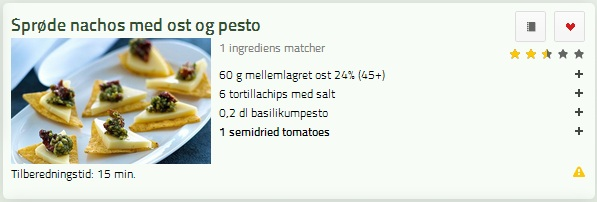
\includegraphics[scale=0.7]{billeder/foodl/opskrift.jpg}
	\capt{Her ses et eksempel på en opskrift, der kan være et resultat på en søgning.}
	\label{fig:foodl-opskrift}
\end{figure}

I toppen af resultatsiden, som er vist på \figref{fig:overblik-resultat}, er der en toolbar, hvorfra brugeren har forskellige muligheder for at manipulere søgningsresultatet. Der er blevet implementeret en toolbar i toppen af siden, der følger brugerens bevægelser mht. at scrolle op og ned. På denne måde behøver brugeren ikke at scrolle helt til toppen for at udføre en handling på søgningsresultatet. 

Figur \ref{fig:foodl-toolbar} præsenterer toolbaren. I venstre side er der en samling af tre knapper, der bruges til at begrænse søgningsresultatet mht. tilberedningstiden. Her er der mulighed for at markere flere af gangen, og default kriteriet er, hvis ingen er markeret, så er alle markeret. Dette betyder, at systemet starter med at vise alle resultater. 
I midten af toolbaren er der et skaleringsværktøj, der kan bruges til at skalere opskrifternes portioner mht. antal personer. Man kan skalere dem ned til en person og op til 10 personer. Vi valgte 10 som maximum, fordi det er relativt let at skalere yderligere, hvis dette er ønsket. 
I højre side af toolbaren er der endnu en samling af tre knapper, men disse benyttes til at sortere opskrifterne. Default er ``relevans''. De to knappesamlinger er forskellige på to måder; hvad de bruges til, og at der kun er mulighed for at markere en knap af gangen ved sorteringsknapperne (højre side) og mulighed for markering af flere af gangen ved afgrænsningsknapperne (venstre side).

\begin{figure}[H]
	\centering
	
\includegraphics[scale=0.7]{billeder/foodl/toolbar.jpg}
	\capt{Systemets toolbar, der er direkte under sidehovedet.}
	\label{fig:foodl-toolbar}
\end{figure}

Ud over toolbaren, så viser \figref{fig:foodl-sidebar} en sidebar, hvilket gør det mulight for brugeren at følge med i, hvad der blev søgt på, og den giver brugeren mulighed for at lave endnu en søgning. Man kan herfra slette og/eller tilføje nye råvaretyper til en ny søgnign. Denne sidebar følger også brugeres scrolling, da det skal være nemt og hurtigt at lave en ny søgning, hvis dette bliver aktuelt.

\begin{figure}[H]
	\centering
	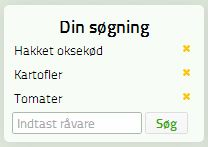
\includegraphics[scale=0.7]{billeder/foodl/sidebar.jpg}
	\capt{Systemets sidebar, der vises ved resultatsiden.}
	\label{fig:foodl-sidebar}
\end{figure}

Hvis en bruger vælger at benytte sig af indkøbslisten, så kan denne tilgås via sidehovedet, ved at trykke på ``indkøbsliste''. I sidehovedet kan man også se, hvor mange varer, der er blevet tilføjet til listen.

Hvis brugere opdager en fejl med en af opskrifterne, så er det muligt at rapportere fejl i systemet.På alle opskrifterne er der en trekantet advarsels-knap i nederste højre hjørne, som kan bruges til at rapportere en fejl vedr. en opskrift. Figur \ref{fig:foodl-fejlrapportering} viser, hvordan det ser ud, når en bruger trykker på rapporteringsknappen ved en opskrift. Der popper en lille boks op, og baggrunden af siden bliver mørk. Her kan man nu specificere, hvad fejlen handler om og give en beskrivelse, inden man vælger at indsende fejlen.

\begin{figure}[H]
	\centering
	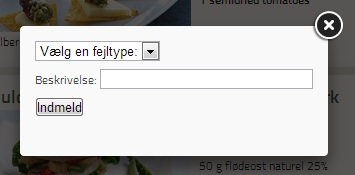
\includegraphics[scale=0.7]{billeder/foodl/fejlrapportering.jpg}
	\capt{Systemets fejlrapportering.}
	\label{fig:foodl-fejlrapportering}
\end{figure}

%området bliver gråt - deb

\subsection{Indkøbsliste}
En indkøbsliste kommer til verden ved, at man i husstanden beslutter sig for at benytte en eller anden form for huskeliste for ting, der skal handles ind. Dette kan være i form af et papir, der ligger et fast sted på bordet eller hænger på opslagstavlen. Denne initierende hændelse kaldes \textit{indkøbsliste oprettet}. Se \figref{fig:indkoebsliste-adfaerd}.

Så længe indkøbslisten ligger på bordet eller et andet sted, kan mange personer komme forbi og tilføje eller fjerne varer på den. Denne tilstand kaldes for \textit{redigeres}. I denne tilstand er det muligt for alle, der kan komme til denne indkøbsliste, at tilføje eller fjerne de varer, der skal handles ind. Man kan \fx fjerne en vare ved at slå en streg over den og give et klart signal om, at denne ikke skal købes. Disse to hændelser hedder \textit{vare fjernet} og \textit{vare tilføjet}. Personen, der tilføjer tekst til indkøbslistene, er herre over, om der skal stå en ingrediens, der består af en mængde, en enhed og en råvare (\fx 1 ltr skummetmælk) eller der blot skal stå råvaren (\fx skummetmælk).

Indkøbslisten kan også indeholde bemærkninger, såsom ``hvis det er på tilbud''. Denne bemærkning kan selvfølgelig også fjernes igen på samme måde som en vare kan fjernes. Disse bemærkninger tilhører en eller flere varer på indkøbslisten, og derfor er hændelsen den samme som ved tilføjelse eller fjernelse af en vare.

Når en person beslutter sig for at tage indkøbslisten med på indkøb, anses indkøbslisten for at være færdig. Det er nu ikke længere muligt at redigere i indkøbslisten, og den afsluttende hændelse indtræffer. 

Ude i supermarkedet kan man købe mange forskellige råvarer. Vi ønsker ikke at overvåge, hvor meget folk har af en ingrediens, og benytter derfor istedet objektet råvare, der ikke indeholder nogen mængde eller enhed. Denne beslutning er taget på baggrund af møde 2 med vores informanter.\todo{Argumenter lidt bedre for valget.}

\begin{figure}[H]
	\centering
	\scalebox{0.8}{
		\subsection{Indkøbsliste}
En indkøbsliste kommer til verden ved, at man i husstanden beslutter sig for at benytte en eller anden form for huskeliste for ting, der skal handles ind. Dette kan være i form af et papir, der ligger et fast sted på bordet eller hænger på opslagstavlen. Denne initierende hændelse kaldes \textit{indkøbsliste oprettet}. Se \figref{fig:indkoebsliste-adfaerd}.

Så længe indkøbslisten ligger på bordet eller et andet sted, kan mange personer komme forbi og tilføje eller fjerne varer på den. Denne tilstand kaldes for \textit{redigeres}. I denne tilstand er det muligt for alle, der kan komme til denne indkøbsliste, at tilføje eller fjerne de varer, der skal handles ind. Man kan \fx fjerne en vare ved at slå en streg over den og give et klart signal om, at denne ikke skal købes. Disse to hændelser hedder \textit{vare fjernet} og \textit{vare tilføjet}. Personen, der tilføjer tekst til indkøbslistene, er herre over, om der skal stå en ingrediens, der består af en mængde, en enhed og en råvare (\fx 1 ltr skummetmælk) eller der blot skal stå råvaren (\fx skummetmælk).

Indkøbslisten kan også indeholde bemærkninger, såsom ``hvis det er på tilbud''. Denne bemærkning kan selvfølgelig også fjernes igen på samme måde som en vare kan fjernes. Disse bemærkninger tilhører en eller flere varer på indkøbslisten, og derfor er hændelsen den samme som ved tilføjelse eller fjernelse af en vare.

Når en person beslutter sig for at tage indkøbslisten med på indkøb, anses indkøbslisten for at være færdig. Det er nu ikke længere muligt at redigere i indkøbslisten, og den afsluttende hændelse indtræffer. 

Ude i supermarkedet kan man købe mange forskellige råvarer. Vi ønsker ikke at overvåge, hvor meget folk har af en ingrediens, og benytter derfor istedet objektet råvare, der ikke indeholder nogen mængde eller enhed. Denne beslutning er taget på baggrund af møde 2 med vores informanter.\todo{Argumenter lidt bedre for valget.}

\begin{figure}[H]
	\centering
	\scalebox{0.8}{
		\subsection{Indkøbsliste}
En indkøbsliste kommer til verden ved, at man i husstanden beslutter sig for at benytte en eller anden form for huskeliste for ting, der skal handles ind. Dette kan være i form af et papir, der ligger et fast sted på bordet eller hænger på opslagstavlen. Denne initierende hændelse kaldes \textit{indkøbsliste oprettet}. Se \figref{fig:indkoebsliste-adfaerd}.

Så længe indkøbslisten ligger på bordet eller et andet sted, kan mange personer komme forbi og tilføje eller fjerne varer på den. Denne tilstand kaldes for \textit{redigeres}. I denne tilstand er det muligt for alle, der kan komme til denne indkøbsliste, at tilføje eller fjerne de varer, der skal handles ind. Man kan \fx fjerne en vare ved at slå en streg over den og give et klart signal om, at denne ikke skal købes. Disse to hændelser hedder \textit{vare fjernet} og \textit{vare tilføjet}. Personen, der tilføjer tekst til indkøbslistene, er herre over, om der skal stå en ingrediens, der består af en mængde, en enhed og en råvare (\fx 1 ltr skummetmælk) eller der blot skal stå råvaren (\fx skummetmælk).

Indkøbslisten kan også indeholde bemærkninger, såsom ``hvis det er på tilbud''. Denne bemærkning kan selvfølgelig også fjernes igen på samme måde som en vare kan fjernes. Disse bemærkninger tilhører en eller flere varer på indkøbslisten, og derfor er hændelsen den samme som ved tilføjelse eller fjernelse af en vare.

Når en person beslutter sig for at tage indkøbslisten med på indkøb, anses indkøbslisten for at være færdig. Det er nu ikke længere muligt at redigere i indkøbslisten, og den afsluttende hændelse indtræffer. 

Ude i supermarkedet kan man købe mange forskellige råvarer. Vi ønsker ikke at overvåge, hvor meget folk har af en ingrediens, og benytter derfor istedet objektet råvare, der ikke indeholder nogen mængde eller enhed. Denne beslutning er taget på baggrund af møde 2 med vores informanter.\todo{Argumenter lidt bedre for valget.}

\begin{figure}[H]
	\centering
	\scalebox{0.8}{
		\input{billeder/tilstandsdiagrammer/indkoebsliste.pdf_tex}}
		\capt{Tilstandsdiagram for klassen indkøbsliste. De afrundede rektangulære bokse med tekst, skal anses som tilstande, som klassen kan have. De pile, der fører til en tilstand, skal anses som hændelser, som kan være skyld i et tilstandsskift. I dette tilfælde har klassen én tilstand (redigeres) og en afsluttende hændelse, der fører klassen ud i en sluttilstand (den sorte prik i den sorte cirkel).}
		\label{fig:indkoebsliste-adfaerd}
\end{figure}}
		\capt{Tilstandsdiagram for klassen indkøbsliste. De afrundede rektangulære bokse med tekst, skal anses som tilstande, som klassen kan have. De pile, der fører til en tilstand, skal anses som hændelser, som kan være skyld i et tilstandsskift. I dette tilfælde har klassen én tilstand (redigeres) og en afsluttende hændelse, der fører klassen ud i en sluttilstand (den sorte prik i den sorte cirkel).}
		\label{fig:indkoebsliste-adfaerd}
\end{figure}}
		\capt{Tilstandsdiagram for klassen indkøbsliste. De afrundede rektangulære bokse med tekst, skal anses som tilstande, som klassen kan have. De pile, der fører til en tilstand, skal anses som hændelser, som kan være skyld i et tilstandsskift. I dette tilfælde har klassen én tilstand (redigeres) og en afsluttende hændelse, der fører klassen ud i en sluttilstand (den sorte prik i den sorte cirkel).}
		\label{fig:indkoebsliste-adfaerd}
\end{figure}
\subsection{Favoritliste}
\label{subsec:brug-favoritliste}

Når der bliver tilføjet en opskrift til en brugers favoritliste, så kan denne opskrift findes under ``favoritter'', som kan findes via sidehovedet i toppen af siden. Et eksempel af en kort opskriftsliste under favoritter kan ses på \figref{fig:overblik-favoritter}.

\begin{figure}[H]
	\centering
	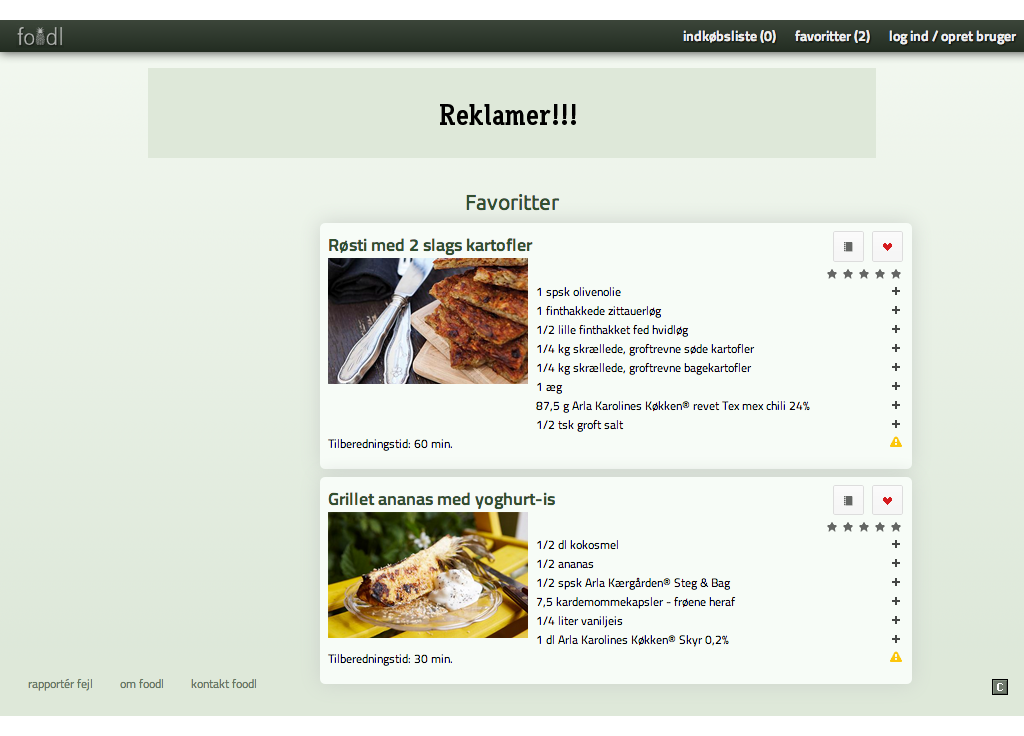
\includegraphics[scale=1]{billeder/foodl/thumbnails/favoritter.png}
	\capt{Denne figur har til formål at give et overblik over systemets favoritside.}
	\label{fig:overblik-favoritter}
\end{figure}

En opskrift bliver tilføjet til favoritlisten ved at trykke på den hjerte-formede knap i øverste højre hjørne af en opskrift. Hvis en opskrift ikke er favoriseret, så er det hjerteformede område i knappen gråt. Når den bliver favoriseret, så bliver hjertet rødt, og dette kan ses i \figref{fig:overblik-favoritter}.

Idéen med favoritlisten er at give brugerne mulighed for at gemme opskrifter, de finder interessante og at de gerne vil bogmærke den til næste gang. De er meget nemmere at finde frem, når man kan finde dem under favoritlisten i stedet for at skulle udføre en ny søgning og prøve at finde den samme opskrift igen.

\subsection{Brugeroprettelse}
\label{subsec:brug-opret}

Alle har mulighed for at oprette en bruger på \Foodl{}. Hvis man har en bruger og logger ind på systemet, så kan man kan gemme sin indkøbsliste og listen over favoritter. Det er dog ikke obligatorisk at have en bruger for at kunne bruge systemet, da vi ikke ønsker at binde brugerne til at oprette noget som helst. Man kan bruge hele systemet, om man har en bruger eller ej.

Man opretter en bruger på samme side, hvor man logger ind på systemet. Dette er præsenteret i \figref{fig:overblik-brugeroprettelse}. Man navigerer til denne side ved at klikke på ``log ind / opret bruger'' i højre side af sidehovedet, som også er synlig på samme figur.

\begin{figure}[H]
	\centering
	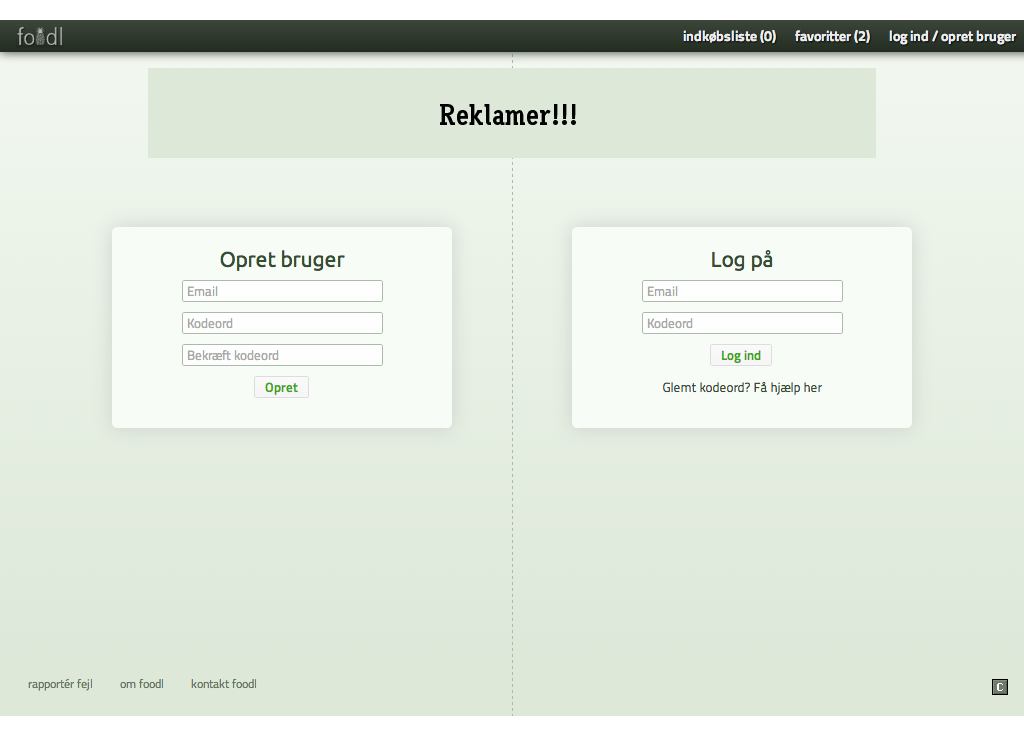
\includegraphics[scale=0.4]{billeder/foodl/thumbnails/opretbrugeroglogind.png}
	\capt{Denne figur har til formål at give et overblik over systemets brugeroprettelsesside.}
	\label{fig:overblik-brugeroprettelse}
\end{figure}

Man skal bruge sin email og en adgangskode for at lave en bruger. Hvis man allerede har en bruger, så skal man blot logge ind med de rigtige oplysninger.

Når man er logget ind, så ændrer sidehovedet sig en smule. Figur \ref{fig:foodl-loggetind} viser, at der nu er mulighed for at gå ind i en menu, der hedder ``indstillinger'' og at logge ud igen.

\begin{figure}[H]
	\centering
	
\includegraphics[scale=0.4]{billeder/foodl/header-login.png}
	\capt{Det ændrede sidehovede, når brugeren er logget ind.}
	\label{fig:foodl-loggetind}
\end{figure}

Hvis man ønsker at skifte sin adgangskode, så sker det ved at trykke på knappen ``indstillinger'' i sidehovedet.

\subsection{Generelt}
Som de fleste andre hjemmesider, så har vi også en ``om'' og en ``kontakt'' side, som kan tilgås fra nederste venstre hjørne af enhver underside af \Foodl{}. Derudover kan man rapportere en generel fejl ved siden, hvis man støder på sådan en. Figur \ref{fig:foodl-formaliteter} viser disse tre knapper.

\begin{figure}[H]
	\centering
	
\includegraphics[scale=0.7]{billeder/foodl/formaliteter.png}
	\capt{I nederste venstre hjørne af systemet kan man rapportere en generel fejl, læse mere om systemet og kontakte udviklerne.}
	\label{fig:foodl-formaliteter}
\end{figure}

Under ``om foodl'' kan brugeren kort læse om dette projekt og om udviklerne bag systemet, altså denne gruppe.

\subsection{Designovervejelser}
\label{subsec:designovervejelser}

Under designet af \Foodl's brugergrænseflade, har vi gjort os nogle designmæssige overvejelser for at øge kvaliteten af programmet. Vi har blandt andet taget højde for følgende principper for god usability\cite[p.~90]{deb}:
\begin{itemize}

\item Visibility
  \begin{itemize}
  \item De vigtigste funktioner har vi valgt altid skal være synlige for brugeren. Det omfatter links til at navigere til siderne \textit{indkøbsliste}, \textit{favoritter}, \textit{log ind / opret bruger} og \textit{forside}. De nævnte links er altid synlige aller øverst på siden i sidehovedet.
  \end{itemize}
  
\item Consistency
  \begin{itemize}
  \item Vi er konsistente med måden hvorpå ting, der kan interageres med, bliver grønne når musen føres over dem. Knapper har den samme firkantede form med svagt afrundede hjørner, grålig baggrund og mørkere grå kanter. Har en knap tekst på sig, er teksten som udgangspunkt grøn. Hvis knappen er blevet trykket i bund og altså er aktiveret, er skriften orange. Hvis en knap er inaktiv og man ikke kan trykke på den, så er kontrasten mellem knappens baggrund, tekst og kant meget lav. Dette kaldes normalt \textit{grayed out}, og er måden man typisk viser at en knap ikke kan trykkes på.
  \item Logoet linker til forsiden, hvilket er ret normalt for de fleste hjemmesider.
  \item En opskrifts vurdering kan læses som 5 stjerner, hvoraf nogle af stjernerne bliver farvet fra venstre mod højre, ligesom folk kender det fra \fx avisers anmeldelser af film.
  \end{itemize}
  
\item Familiarity
  \begin{itemize}
  \item Vi benytter symboler folk i forvejen kender, som \fx krydset man trykker på for at slette en råvare man har indtastet eller når man vil slette en ingrediens fra indkøbslisten. Når man skal tilføje en ingrediens til indkøbslisten trykker man på et plus-symbol, som ofte forbindes med at tilføje noget.
  \item Når en søgning er sat i gang, så vises en cirkulær animation, som ofte bruges når en proces, der kan tage et stykke tid, er i gang.   
  \end{itemize}
  
\item Affordance
  \begin{itemize}
  \item Vi har forsøgt at designe \Foodl's logo, samt forsiden hvor logoet præsenteres, på en sådan måde at folk med det samme får et indtryk af hvad systemet kan. Logoets tekst, \textit{Foodl}, får tankerne over på mad, hvilket yderligere forstærkes af at det ene ``o'' er udskiftet med en ananas. Navnet Foodl minder en smule om Google, og har til formål at lede folks tanker i retning af en søgemaskine, hvilket yderligere forstærkes af sidehovedet og forsidens design, der minder en hel del om Googles.  
  \item Når man skal favorisere en opskrift, altså tilkendegive at man synes om denne, så skal man trykke på en knap med et  hjertesymbol. Hjertet skal gerne give folk en ide om, at man altså skal trykke på knappen hvis man synes om opskriften.
  \item Indkøbslisten ligner et rigtig linieret A4-papir. Varer på listen vises med en skrifttype, der ligner håndskrift, dog ikke i så høj grad at det bliver svært at læse teksten. Vi benytter altså en metafor her, ved at tage et kendt objekt og mappe det til noget virtuelt, der ser ud og fungerer på samme måde.
  \item En stjerne bliver associeret med noget godt. Derfor viser vi et antal stjerner ved en opskrift, for at folk skal forbinde det med hvor god en opskrift er.
  \end{itemize}
  
\item Navigation - vi har forsøgt at gøre navigation imellem \Foodl's sider mere enkel ved at bruge flere forskellige elementer
  \begin{itemize}
  \item Et sidehovede, sørger for at de overordnede muligheder for at navigere imellem sider altid er synlig.
  \item Hvis man ikke er logget ind, kommer der en sort, firkantet boks frem med teksten “Husk at oprette en bruger for at gemme din indkøbsliste og favoritter”. I boksen er der en pil, der peger lige netop på det link i sidehovedet man skal trykke på for at oprette en bruger.
  \item Når man har udført en søgning får man aller først vist alle resultater. Derefter kan man sortere og begrænse søgningen. Dette opfylder designprincippet \textit{Overblik først, derefter detaljer}.
  \end{itemize}
  
\item Control - vi giver viden om hvad han kan kontrollere
  \begin{itemize}
    \item Når musen er over en knap, der kan interageres med, bliver knappens baggrund grøn. Så ved man at man kan trykke på knappen, og på samme måde finder man hurtigt ud af at en slider kan trækkes i.
    \item Når der trækkes i slideren, der skalerer opskrifterne i et søgeresultat, så ændres antal personer og ingrediensernes mængder sig med det samme, og ikke først når slideren er sluppet. På den måde får brugeren bedre kontrol og kan hurtigt ramme den rigtige skalering.
    \item Ting, der ikke kontrolleres ser udhviskede ud.
  \end{itemize}
  
\item Feedback - vi giver brugeren feedback, så han ved at systemet har reageret på hans forespørgsler, og fortæller ham når noget er gået galt eller hvis han har lavet en fejl.
  \begin{itemize}
  \item En animation af en cirkulær bevægelse viser at en søgning er i gang. På den måde tror brugeren ikke at han har klikket ved siden af en knap, hvis søgning blot tager lidt længere tid end forventet.
  \item En besked popper op på siden når brugeren skal have feedback. Det kan \fx være når brugeren har oprettet en bruger eller har indtastet en forkert kode i et forsøg på at logge ind.
  \end{itemize}

\item Revocery
\begin{itemize}
  \item Hvis en bruger har glemt sin kode, kan han få den tilsendt igen.
\end{itemize}

\item Style
\begin{itemize}
  \item Vi har brugt HTML og CSS til at opbygge et, i vores øjne, flot og attraktivt design.
\end{itemize}

\item Conviviality
\begin{itemize}
  \item Hvis en bruger laver en fejl, så forholder vi os relativt roligt og viser brugeren en lille tekstmeddelelse med feedback. Vi afspiller ikke en lyd, der får folk til at spilde kaffen.
  \item Når noget er gået galt, giver vi ikke brugeren skylden for dette direkte. Hvis en person forsøger at logge ind uden at have indtastet gyldig email-adrasse, så skriver vi blot \textit{Angiv en email-adresse}, i stedet for \textit{Du har indtastet en forkert email-adresse}. På samme måde med alle fejlmeddelelser, bebrejder vi ikke brugeren direkte.
  \item
\end{itemize}

\end{itemize}